\section{Kanalcodierung \schaum{282-11}} 
\begin{center}
	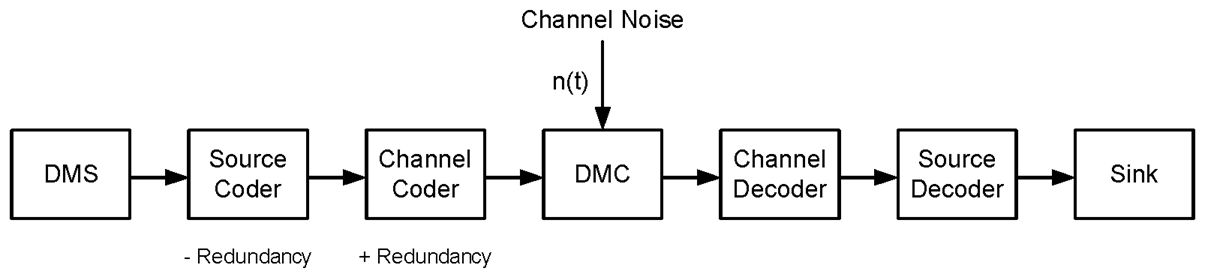
\includegraphics[width=11cm]{../NaT2/bilder/11_channel_coding_blockdiag.png}
\end{center}

Mit der Kanalcodierung können \textbf{Übertragungsfehler erkannt} und \textbf{beseitigt} werden.
Dies geschieht durch beifügen geeigneter \textbf{Redundanz}. \\
Je nachdem wieviel Redundanz in dem Code beinhaltet ist, handelt es sich um einen \textit{error-detecting
code} oder sogar um einen \textit{error-correcting code}.

\subsection{Kanalkodierungstheorem - Shannon \schaum{282-11.2B}}
Gegeben seien DMS mit Entropie $H(X)$ und DMC mit Kanalkapazität $C_s$. 

\begin{itemize}
  	\item Für $H(X) < C_s$ kann mit geeigneter Kanalcodierung die \textbf{Fehlerrate} der
  	Übertragung \textbf{beliebig klein} gemacht werden. 
	\item Für $H(X) > C_s$ ist eine \textbf{fehlerfreie} Übertragung \textbf{nicht möglich}.
\end{itemize}
%Wenn man jedoch $n = \frac{H(x)}{C_s}$ Bits (binary digits) pro Symbol der Datenquelle bei
%geeigneter Codierung überträgt kann die Übertragung mit beliebig kleiner Fehlerrate erfolgen. \\ \\
Bitfehler in der Übertragung verunmöglichen einen zuverlässigen Informationsaustausch nicht,
sondern beschränken die nutzbare Übertragungsrate - je mehr Fehler desto mehr Übertragungsrate
wird für die Fehlerkorrektur benötigt. \\

\subsection{Blockcodes}
Hierbei wird aus (relativ kleinen) Datenblöcken mit \boldmath$k$ \textbf{Eingangssymbolen} Codes mit
je $n$ \unboldmath \textbf{Ausgangssymbolen} (mit $n > k$) generiert. Wobei jeder dieser Blöcke
separat Codiert wird. Man spricht dann auch von einem $(n,k)$-Code. Beispielsweise handelt es
sich bei einer RS232-Übertragung mit 8 Daten- und 1 Paritätsbit um einen $(9,8)$-Code. \\
\hspace*{0.5cm} \parbox[c][1cm]{5cm}{\textbf{Coderate} $R_c = \frac{k}{n}$}\\
In unserem Fall (binär) kann ein Symbol zwei Zustände aufweisen. Diese Zustände sind in der binären
Menge ($K=\{0,1\}$) definiert.
Folgende mathematische Operatoren werden auf diese Menge angewendet:
\begin{itemize}
  \item Modulo-2-Addition: ``$\oplus$'' = logisches XOR $\quad\Rightarrow
  \quad(0,0)=0\;/\;(0,1)=1\;/\;(1,0)=1\;/\;(1,1)=0$
  \item Multiplikation: ``$\cdot$'' = logisches AND
\end{itemize}


\subsection{Lineare Blockcodes \formelbuch{283-11.4}}
Ein Code gilt als linear, falls die Summe jeder beliebigen Codeworte ($\vec{a},\vec{b}$) wiederum auch ein
Codewort ($\vec{c}$) ist. 
$$\vec{a} = (a_1, a_2, \ldots, a_n) \quad \text{ und } \quad \vec{b} = (b_1, b_2, \ldots, b_n) \quad
\Longrightarrow \quad \vec{c} = \vec{a} \oplus \vec{b} = (a_1 \oplus b_1, a_2 \oplus b_2, \ldots, a_n \oplus b_n)$$

Wegen: $\quad \vec{a} \oplus \vec{a} = \vec{b} \oplus \vec{b} = 0 = (0,0,\ldots,0) \quad$, gilt \textbf{zwingend}, dass
zu jedem linearen Code der \textbf{Nullvektor} $\vec{0}$ gehört. Jeder Code der mit einer Generatormatrix
gebildet werden kann ist ein linearer Code.

\subsubsection{Hamming-Gewicht, (minimale) Hamming-Distanz \formelbuch{283-11.4.C,D}}
\renewcommand{\arraystretch}{1.4}
\begin{tabular}[c]{ p{5.0cm}  p{5.0cm} p{9cm} }
	\textbf{Hamming-Distanz}:
	& $d(\vec{a},\vec{b}) = w(\vec{a} \oplus \vec{b})$
	& \textbf{Anzahl unterschiedliche Stellen} zweier Codeworte \\
	\textbf{Minimale Hamming-Distanz}\textcolor{red}{*}:
	& $d_{min} = \min[d(\vec{a},\vec{b})] \underbrace{= \min{[w(\vec{c})]}}_{\text{wenn lin. Code C}}$
	& \parbox[c]{9cm}{\textbf{Minimum} der Distanz aller mög. Codewort-Paarte\\
	Bei lin. Code: \textbf{Kleinstes} Hamming-Gewicht aller Codeworte} \\
	\textbf{Hamming-Gewicht}: 
	& $w(\vec{c}) = d(\vec{c},0)$
	& \textbf{Anzahl 1} eines Codeworts exkl. Nullvektor
\end{tabular}
\renewcommand{\arraystretch}{1} \\
\textcolor{red}{*}: Die Minimale Hamming-Distanz kann auch mittels der Paritätsprüfmatrix
\verweiskurz{paritycheckmatrix} berechnet werden.


\subsubsection{Fehlererkennung- und Fehlerkorrektur-Möglichkeiten}
Durch die minimale Hamming-Distanz ist die Anzahl korrigierbarer und detektierbarer Fehler
gegeben. \\
\renewcommand{\arraystretch}{1.4}
\begin{tabular}[c]{ p{5.5cm}  p{13cm} }
	Anzahl \textbf{detektierbare} Fehler & $t_d = d_{min} - 1$ \\
	Anzahl \textbf{korrigierbare} Fehler & $t_c = \frac12 (d_{min} - 1) = \frac12 t_d$
\end{tabular}
\renewcommand{\arraystretch}{1} \\

\begin{minipage}{7.5cm}
	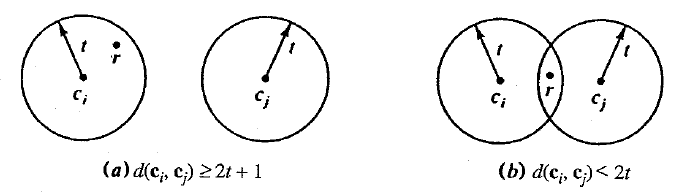
\includegraphics[width=7cm]{../NaT2/bilder/11_hamming_distance.png}
\end{minipage}
\begin{minipage}{11.5cm}
	Nebenan eine geometrische Veranschaulichung: Je mehr unterschiedliche Stellen (Hamming-Distanz)
	zwei Codeworte haben, desto weiter entfernt liegen die beiden Kreise - Abb. (a). Liegt deren
	Abstand (Hamming-Distanz) jedoch unter dem doppelten Radius ($< 2$), so kann der Decoder nicht mehr
	eindeutig feststellen, zu welchem ``Kreis'' das empfangene Zeichen gehört - Abb. (b).
\end{minipage} 

\subsection{Systematische Codes}
\begin{minipage}{5.5cm}
	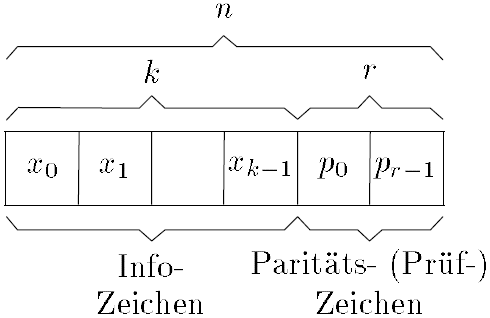
\includegraphics[width=5cm]{../NaT2/bilder/11_systematic_code.png}
	\centering geordnet-systematischer Code
\end{minipage}
\begin{minipage}{12.8cm}
	Ein Code gilt als systematisch, sobald alle \textbf{Datenbits} $d_i$ an irgend einer Stelle des Codes $c_i$
	\textbf{unmodifiziert} vorkommen. Die nötigen Prüfzeichen werden meist am Ende
	der Datenbits angefügt und können wenn gewünscht ausgewertet werden. Anwendungsbeispiele:
	\begin{itemize}
    	\item CRC (Cycle Redundancy Check) bei MP3, JPEG, \ldots
    	\item Parity Check bei RS232
  	\end{itemize}	
	Die Coderate $R_C$ Ist das Verhältnis zwischen Codelänge und Nutzdaten: $\frac{k}{n}$
\end{minipage} 

\subsubsection{Generatormatrix G \schaum{285-11.4.F}}
Mittels der \textbf{Generatormatrix} $G$ kann das jeweilige \textbf{Codewort} $\vec{c}$ aus dem \textbf{Datenwort} $\vec{d}$
generiert werden. Dimensionen: $\textcolor{blue}{[H\times B]}$
$$ \vec{c}\textcolor{blue}{_{[1 \times n]}} = \begin{bmatrix} c_1 & c_2 & \ldots & c_n \end{bmatrix} =
\vec{d}\textcolor{blue}{_{[1 \times k]}} \cdot G\textcolor{blue}{_{[k \times n]}} =
                \begin{bmatrix} d_1 & d_2 & \ldots & d_k \end{bmatrix} 
				\cdot \begin{bmatrix} 
					1 & 0 & \ldots & 0 & p_{11} & p_{21} & \ldots & p_{m1} \\              
					0 & 1 & \ldots & 0 & p_{12} & p_{22} & \ldots & p_{m2} \\
					\vdots & \vdots & \vdots & \vdots & \vdots & \vdots & \vdots & \vdots \\
					0 & 0 & \ldots & 1 & p_{1k} & p_{2k} & \ldots & p_{mk} \\
				\end{bmatrix} \overset{\textcolor{red}{*}}{=} \vec{d} \cdot [I\textcolor{blue}{_{[k \times k]}} \;
				P^T\textcolor{blue}{_{[k \times (n-k)]}}] $$ Bei $P^T$ handelt es sich um die trasponierte
				Paritätsmatrix $P$, bei $I_k$ um die $[k \times k]$- Einheitsmatrix (\emph{I}dentität). \\
\textcolor{red}{*}: Das letzte Gleichheitszeichen gilt nur, falls
es sich um einen systematischen Code handelt. Ansonsten ist auch der linke Teil der Generatormatrix
nicht genau mit der Einheitsmatrix ``gefüllt''.

\subsubsection{Paritätsprüfmatrix H \schaum{285-11.4.G}} \label{paritycheckmatrix}
Die Paritätsprüfmatrix $H$ dient zur \textbf{Erkennung von Übertragungsfehlern}. 
$$H\textcolor{blue}{_{[(n-k) \times n]}} = \begin{bmatrix}P & I_{n-k}\end{bmatrix} \Rightarrow
H^T\textcolor{blue}{_{[n \times (n-k)]}} =
\begin{bmatrix} P^T \\ I_{n-k}\end{bmatrix} 
\qquad \qquad 
G \cdot H^T = \begin{bmatrix}I_k & P^T\end{bmatrix} \cdot 
 \begin{bmatrix} P^T \\ I_{n-k}\end{bmatrix} = P^T \oplus P^T = 0
	\qquad \qquad
	\vec{c} \cdot H^T = \vec{d} \cdot G \cdot H^T = \vec{0}
	 $$
Die Multiplikation der Generatormatrix mit der transportierten Paritätsprüfmatrix ergibt eine 
$[k \times (n-k)]$-\textbf{Nullmatrix}. Somit ergibt die Multiplikation von einem
\textbf{gültigen Codewort} und der transportierte Paritätsprüfmatrix immer ein $[1
\times (n-k)]$-\textbf{Nullvektor}. \\
Die \textbf{minimale Hamming-Distanz} $d_{min}$ vom Code $C$ entspricht genau der minimalen
nötige Anzahl irgendwelcher Zeilen von $H^T$, sodass deren \textbf{Linearkombination Null} ergibt.


\subsubsection{Auswertung des Fehlersyndroms s \schaum{286-11.4.H}}
Das \textbf{Fehlersyndrom} $s$ erlaubt die Erkennung und eventuelle Korrektur von Übertragungsfehlern.
Angenommen das empfangene Codewort $c_r$ ist mit einem \textbf{Fehlermuster} $e$ versehen.
$$\vec{c}_r = \vec{c} \oplus \vec{e} \qquad \qquad \vec{s}\textcolor{blue}{_{[1 \times (n-k)]}} = \vec{c}_r \cdot H^T = \vec{c}
\cdot H^T \oplus \vec{e} \cdot H^T = \vec{e} \cdot H^T$$

Bei einem Einzelfehler entspricht das Fehlersyndrom $s$ gerade einer \textbf{Zeile von }
\boldmath$H^T$\unboldmath . Die \textbf{Zeilennummer} $i$ entspricht genau der \textbf{fehlerhaften
Position} im Code. Um den Code zu korrigieren wird die entsprechende Position invertiert.
$$ \vec{e} = \begin{bmatrix} \underbrace{0}_{1} & \ldots & 0 & \underbrace{1}_i & 0 & \ldots & 0\end{bmatrix} $$ 
Sind \textbf{alle} Zeilen von $H^T$ \textbf{unterschiedlich} entspricht dies \boldmath $d_{min}
\geq 3$ \unboldmath . 
Zugleich kann bei Einzelfehlern aus $s$ das \textbf{Fehlerbit} $e_i$ \textbf{eindeutig} bestimmt und das 
empfangene Codewort $c_r$ \textbf{korrigiert} werden. \\

\textbf{Hamming-Schranke}\\
\begin{minipage}{12cm}
	Ein $(n,k)$-Blockcode kann bis zu t Fehler korrigieren, falls $n$
	und $k$ die nebenstehende Ungleichung erfüllen. Diese Bedingung ist notwendig aber \textbf{nicht
	hinreichend}. Massgebend sind die Linearität und die minimale Hamming-Distanz. \\
	Gilt das Gleichheitszeichen, so handelt es sich um einen sog. \textbf{perfekten Code}. \\
	Einzelfehler korrigierende perfekte Codes nennt man \textbf{Hamming-Codes}.
\end{minipage} 
\begin{minipage}{7cm}
	$$ \qquad 2^{n-k} \geq \sum\limits_{i=0}^{t} \binom{n}{i} \quad$$ \\
	$$ \text{mit} \quad \binom{n}{i} = \dfrac{n!}{(n-i)! i!} \quad \text{oder TR: \textbf{nCr(n,i)}}$$
\end{minipage}

\newpage

\subsection{Zyklische Blockcodes \schaum{286-11.5}}
Coder und Decoder von gewissen \textbf{linearen Blockcodes} sind ab einem Umfang von $n \gg 1$ und
$k \gg 1$ sehr \textbf{aufwendig} zu realisieren. \\
\textbf{Abhilfe} schaffen die zyklischen Blockcodes - eine \textbf{Untergruppe} der linearen Blockcodes -
welche es erlauben mit einem \textbf{kleinen Hardwareaufwand} Coder und Decoder zu realisieren. 
$$ \text{einfache: }\sigma(\vec{c}) = \vec{c}^{(1)} = (c_{n-1}, c_0, c_1, \ldots, c_{n-2}) \qquad 
 \text{2-fache }\sigma^2(\vec{c}) = \sigma\{\sigma(\vec{c})\}= \vec{c}^{(2)} = (c_{n-2}, c_{n-1}, c_0, \ldots, c_{n-3}) \qquad
 \text{n-fache }\sigma^n(\vec{c}) = \vec{c} $$
Wenn die \textbf{zyklische Verschiebung} $\sigma (c)$ eines Codeworts $\vec{c} = (c_0, c_1, \ldots,
c_{n-1})$ wiederum ein \textbf{gültiges Codewort} $\vec{c}$ ergibt, so handelt es sich bei dem Code um
einen linearen Blockcode.


\subsubsection{Code-Polynom c(x), Modulo-2-Polynom Arithmetik \schaum{287-11.5.B}}
Zur mathematischen Behandlung werden zyklische Codes als Polynome dargestellt, wobei die
Koeffizienten $c_i$ jeweils der binären Menge $K=\{0,1\}$ angehören.
$$ \vec{c} = (c_0, c_1, c_2, \ldots,
c_{n-1}) \quad \Longleftrightarrow \quad c(x) = c_0 + c_1 x + c_2 x^2 + \ldots + c_{n-1} x^{n-1} 
\qquad \qquad \text{Bsp.: } \vec{c} = (1, 0, 0, 1, 1, 0) \quad \Longleftrightarrow \quad c(x) = 1 + x^3 +
x^4$$

\textit{Addition, Subtraktion, Multiplikation:} \\
Die Polynome können auf die \textbf{übliche} Weise \textbf{multipliziert} und \textbf{addiert} werden,
\textbf{ausser} bei \textbf{gleichem Exponent} ergibt eine \textbf{Addition Null}.
Im binären Fall sind die Modulo-2-\textbf{Addition} und
-\textbf{Subtraktion identische} Operationen. 
$$ mod2(x^k + x^k) = 0 \qquad mod2(x^k - x^k) = 0 \qquad mod2(0 + x^k) = x^k \qquad mod2(0 - x^k) = x^k$$

\textit{Division:}\\
Die Modulo-2-Division stellt eine etwas \textbf{spezielle} Rechnung dar.
Eine Divison von \boldmath$f(x)$ durch $h(x)$ ergibt den Quotienten $q(x)$ mit Rest $r(x)$
\unboldmath . 
$$ \dfrac{f(x)}{h(x)} = q(x) + \dfrac{r(x)}{h(x)} \qquad \Longleftrightarrow \qquad \boxed{f(x) = q(x)
\cdot h(x) + r(x)}$$ 
Um $q(x)$ und $r(x)$ zu berechnen muss man die \textbf{übliche Polynomdivision} anwenden, \textbf{jedoch}
bei Addition und Subraktion zwischen den Koeffizienten Modulo-2-Addition anwenden. \\ 
Der \textbf{Modulo Operator} stellt eine vereinfachte Schreibweise dar, die jedoch teils auch
\textbf{verwirrend} sein kann.
$$ (1) \quad r(x) = f(x) \mod{h(x)} \qquad \qquad 
(2) \quad a(x) = b(x) \mod{h(x)} \qquad \qquad 
(3) \quad x^n = 1 \mod{(1 + x^n)}$$
Gleichung 1 bedeutet, dass $f(x)$ geteilt durch $h(x)$ den Rest $r(x)$ ergibt. \\
Gleichung 2 soll ausdrücken, dass beide Polynome $a(x), b(x)$ durch $h(x)$ dividiert den selben
Rest ergeben. \\
Gleichung 3 will sagen, dass (für ein beliebiges $n$) $x^n$ durch $(1 + x^n)$ geteilt, denn Rest
$1$ ergibt. \\
Somit ist das \textbf{Chaos} perfekt. Folgendes ist zu beachten um Klarheit zu schaffen:\\
Generell steht der Modulo Operator \textbf{immer} auf der \textbf{rechten Seite der Gleichung}. 
Das \textbf{Rest-Polynom} $r(x)$ ist immer dasjenige mit dem \textbf{kleinsten Grad
}($\PolyGrad[r \left( x \right)] < \PolyGrad[h \left(x \right)]$ und
$\PolyGrad[r \left(x \right) ] < \PolyGrad[f \left( x \right)]$).
\\

\textit{Zyklische Verschiebung} \\
Eine $i$-\textbf{fache zyklische Verschiebung} eines Polynoms erfolgt in drei Schritten:
$$ c^{(i)}(x) = c(x) x^i \mod{(1+x^n)}$$
\begin{enumerate}
  \item Multiplikation des Codepolynoms $c(x)$ mit $x^i$
  \item Division mit $(1+x^n)$
  \item Divisionsrest $r(x)$ entspricht gerade $c^{(i)}(x)$
\end{enumerate}

\subsubsection{Generator-Polynom g(x) \schaum{287-11.5.C}}
Jeder $[n,k]$ zyklische Code kann mit Hilfe des Generator-Polynoms $g(x)$ (vom Grade $(n-k)$)
durch Multiplikation mit dem Daten-Polynom $d=d_0 + d_1x + \ldots + d_{k-1}x^{k-1}$ gebildet werden.
$$ g(x) = \textcolor{blue}{g_0} + g_1 x + g_2 x^2 + \ldots + \textcolor{blue}{g_{n-k}} x^{n-k}
\quad \text{mit (} \textcolor{blue}{g_{n-k} = g_0 = 1} \text{) } \qquad \Longrightarrow \qquad
c(x) = d(x) \cdot g(x)$$
Das Generatorpolynom wird durch \textbf{Modulo-2-Faktorzerlegung} (sehr kompliziert) gewonnen: 
$$ (x^n + 1) = q(x) \cdot \textcolor{purple}{g(x)} \qquad \qquad \text{Bsp.: } \quad (n=7,k=4) \quad
\Rightarrow \quad (x^7 + 1) = (x+1)\textcolor{purple}{(x^3+x+1)(x^3+x^2+1)}$$ Jedes Polynom der
Faktorzerlegung vom Grad ($n-k$) mit $g_{n-k} = g_0 = 1$ kann als Generatorpolynom verwendet
werden. Mittels \textbf{\matlab{cyclpoly(n,k,'all')}} können alle möglichen Generatorpolynome
erzeugt werden.
% einige generatormatritzen mittels matlab einfügen?!?

%\subsubsection{Paritätsprüf-Polynom h(x) \schaum{288-11.5.D}}

\subsubsection{Syndrom-Polynom s(x) \schaum{288-11.5.E}}
\begin{minipage}{13.1cm}
Das Fehlersyndrom $s(x)$ (vom Grad ($n-k$)) dient zur \textbf{Ermittlung von Übertragungsfehlern}.
Enthält das empfangene Codewort $c_r(x)$ ein \textbf{Fehlermuster} $e(x)$, so entspricht der
Rest der Division (Decodierung) dem sog. Fehlersyndrom $s(x)$.
$$ c_r(x) = c(x) + e(x) \quad \qquad \text{Fehlersyndrom: } \boxed{s(x) = c_r(x) \quad \mod{g(x)}} $$
% $$ d(x) = \dfrac{c(x)}{g(x)} \Longrightarrow \dfrac{c_r(x)}{g(x)} = d(x) + \dfrac{s(x)}{g(x)}$$
$$ \text{Aus } c(x) = d(x)\cdot g(x) \text{ folgt } s(x) = e(x) \mod{g(x)}$$

	Die Fehlermuster $e(x)$ und die dazugehörigen Fehlersyndrome $s(x)$ werden in einer
\textbf{Tabelle} erfasst, sodass bei einem Syndrom $s(x)$ gerade auf das entsprechende Fehlermuster $e(x)$
geschlossen und dieses korrigiert werden kann.
\end{minipage} 
\begin{minipage}{0.3cm}
$\quad$
\end{minipage}
\begin{minipage}{7cm}
	\begin{tabular}{| p{1.8cm} | p{2.8cm} |}
  		\hline
  			Fehler $e(x)$ & Fehlersyndrom $s(x)$ $= e(x)  \mod{g(x)} $ \\
  		\hline
  			$1$	&	$1 \mod{g(x)}$ \\
  			$x$	&	$x \mod{g(x)}$ \\
  			$x^2$	&	$x^2 \mod{g(x)}$ \\
  			$\vdots$ & $\vdots$ \\
  			$1 + x$ &	$1+x \mod{g(x)}$ \\
  			$1 + x^2$ &	$1+x^2 \mod{g(x)}$ \\
  			$\vdots$ & $\vdots$  	\\		
  		\hline
  	\end{tabular}
\end{minipage}

Ist der \textbf{empfangene Code korrekt}, so ist das Fehlersyndrom \boldmath$s(x) =
0$\unboldmath.\\ \\
Für einen zyklischen Code mit minimaler Hamming-Distanz $d_{min}$ hat jedes
Fehlermuster mit Hamming-Gewicht $< \frac12 d_{min}$ ein ganz \textbf{charakteristisches, eindeutiges Fehlersyndrom}, welches nur vom Fehler $e(x)$
abhängig ist.

\subsubsection{Codierung - Multiplikation \schaum{289-11.5.F}}
\begin{minipage}{9cm}
	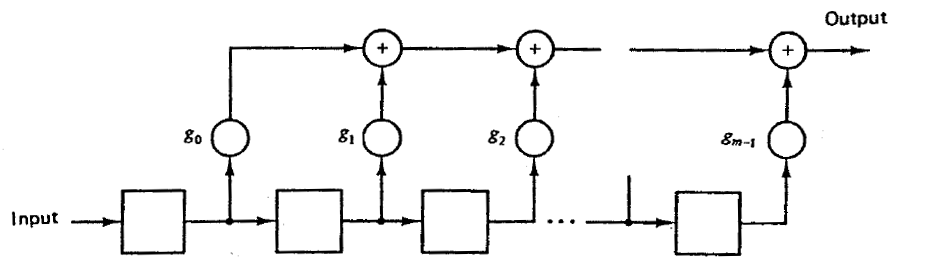
\includegraphics[width=9cm]{../NaT2/bilder/11_cyclic_coder_multiplication.png}
\end{minipage}
\begin{minipage}{9.5cm}
	Zur Codierung der Datenworte dient ein m-faches ($m = n-k$) \textbf{Schieberegister}. \\
	Das Datenwort muss mit \textbf{Zero-Padding} (konstante Länge, d.h. vorne mit 0 aufgefüllt) vorhanden sein.
	Zudem gilt in der nebenstehenden Form ``\textbf{LSB first}" ($d_0$) . Ist ``MSB first''($d_{k-1}$) gewünscht, so muss
	lediglich die Reihenfolge von $g_i$ getauscht werden.
\end{minipage}

\subsubsection{Decodierung - Division \schaum{289-11.5.F}}
\begin{minipage}{9.4cm}
	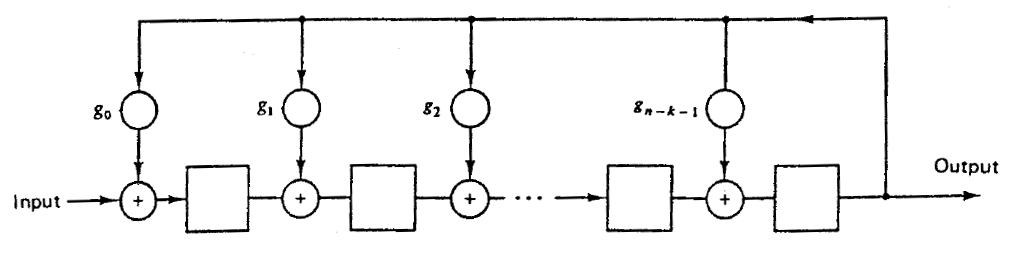
\includegraphics[width=9cm]{../NaT2/bilder/11_cyclic_decoder_division.png}
\end{minipage}
\begin{minipage}{9cm}
	Die Decodierung der Codeworte erfolgt durch ein (n-k-1)-faches \textbf{Feedback-Schieberegister}.\\
	Nach $n$-Taktzyklen entspricht der Ausgang dem Datenwort $d$ und der Inhalt des Schieberegisters
	dem Fehlersyndrom (Rest der Division). \\ 
	Das Codewort muss in der nebenstehenden Form mit \textbf{``MSB first''} ($c_{n-1}$) vorliegen.
\end{minipage}


\subsubsection{Realisierung eines systematischen Codes}
Ein zyklischer Blockcode kann immer in eine systematische Form gebracht werden, ohne dass die
Hamming-Distanz verändert wird oder die zyklische Eigenschaft verloren geht.
Die Matrix G eines nicht-systematischen zyklischen Codes kann durch die Zeilen $g(x), x\cdot g(x), \ldots, x^{k-1}\cdot g(x)$ gebildet werden. 
$\Rightarrow$ Durch Zeilenkombination (Additionen) kann G in eine systematisch Form gebracht werden. Oft ist es üblich den systematischen Teil (Einheitsmatrix) im rechten Teil der Matrix G unterzubringen.\\
\hspace*{0.5cm}$ c(x) = p(x) + x^{n-k}\cdot d(x)$\\
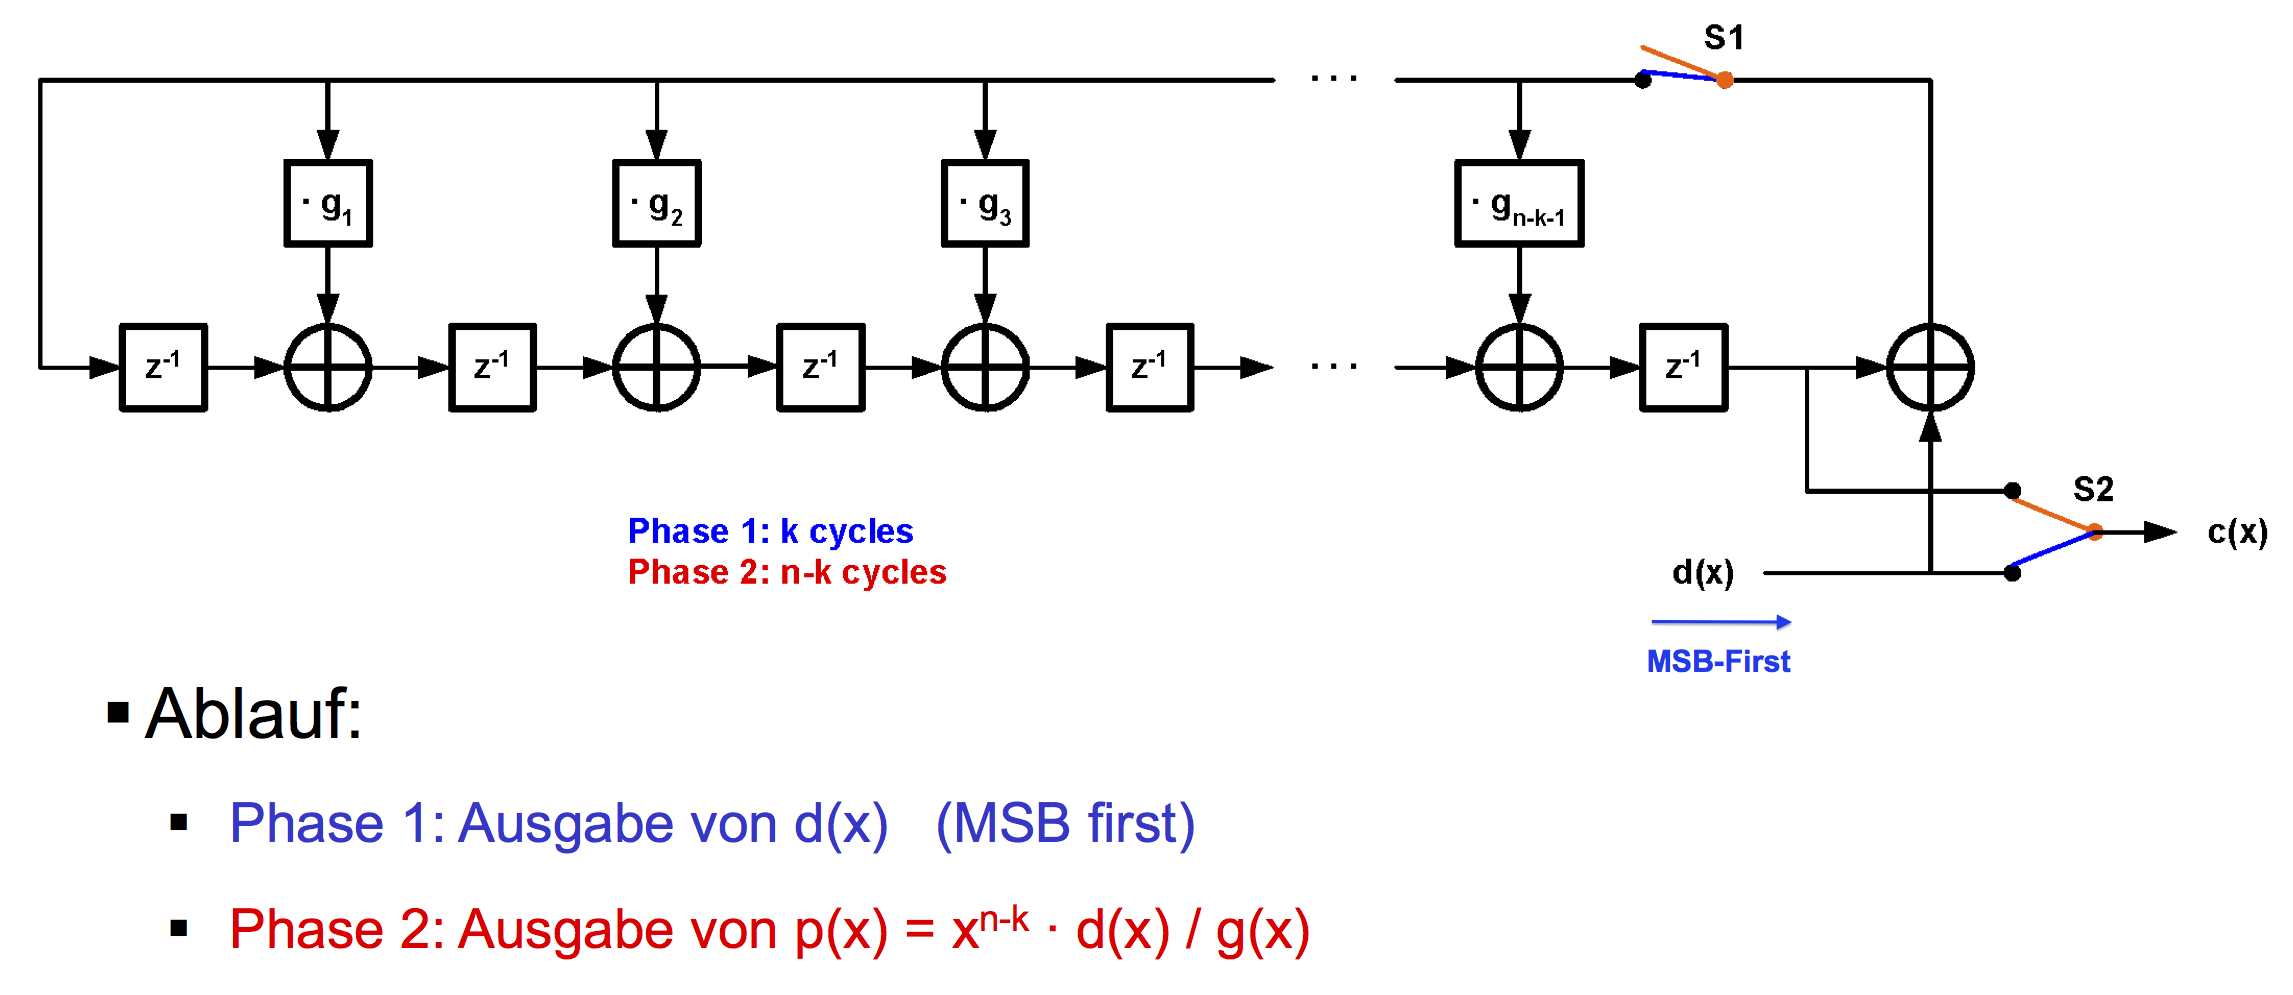
\includegraphics[width = 12cm]{./bilder/11_cyc_hw_imp_sys_code}

\subsection{Faltungscodes \schaum{290-11.6}}
\textit{Nicht prüfungsrelevant!}\\ \\
Hierbei werden ganze Daten Streams codiert. Der Code hängt hier nicht nur vom aktuellen Datenblock
ab, denn der Codierer bezieht auch noch einige vorgängige Blöcke in die Codierung mit ein.
